\section{Introduction}
During the last years the usage of smart-wearables (particularly smartwatches) has become more and more common with a number of 337 million units sold in 2019 and a forecast in sales of up to 527 million units by 2024 \cite{tenzer}.
With that also comes a natural demand in data protection due to the many sensors built in these devices due to their ability to capture sensible personal information (e.g. health informations) and additionally the fact that smart devices also can now be used for many kinds of financial actions.\newline
Since most wearables are connected to either the distributors or the respective mobile phones virtual assistant they should contain sensors for on one hand sound conduction and on the other hand audio recording.\newline
Based on these conditions smartwatches could be used in combination with biometric authentication mechanics.\newline
In general biometric authentication can be split into behavioural and physiological biometrics as well as authentication can be split into implicit and explicit methods. The exact characteristics will be described as follows: 
\subsection{Biometrics}
\textit{Biometrics} (as in the greek terms \textit{bios} and \textit{metrikos}) describes the utilization of an individuals physical traits or behaviour to clearly identify one from others. Contrary to the more known verification methods as PINs, passwords or ID-cards biometric identification does not rely on tokens or knowledge which could easily be forgotten or stolen, rather than unique personal traits like fingerprints, face or the specific way someone interacts \cite[chpt. 1.1]{jain2007handbook}\cite{delac2004survey}. Therefore the individual wishing to authenticate first has to enrol one specific trait of hers to the biometric system. Based on this sample data the system generates an authentication template which is later on used to authenticate against.\newpage
When someone now wants to register using the system he provides the trait wanted to the system from which then a new sample is generated. The generated sample then is compared to the template \cite{alsaadi2015physiological}.\newline
Tests used for this comparison can be designed based on two different points of view. First of positive identification or authentication and second negative identification/authentication. Negative authentication presumes the given sample is from an unknown user whereas the sample in a positive authentication scenario should be by a known user \cite{wayman2005introduction}.
As already stated above biometric authentication uses an individuals personal traits as authentication tokens. Based on the kind of trait and the methods how they could be provided the general term of biometrics can be further divided into \textit{behavioural} and \textit{physiological} biometrics. How each of them is defined exactly will be defined in the following.
\subsubsection{Behavioural Biometrics} Behavioural biometrics refers to authentication systems in which process of authentication is conducted with the use of primarily gestures or other actions able to be performed in everyday life. Usable features for this purpose are e.g. gait or keystroke analysis. Advantages this kind of biometrics has are e.g. that there is no direct need for special hardware since it is mostly used with smart wearables or mobile phones who each have the required sensors built in. Another advantage would be that the data required must not be collected actively by the user but is recorded passively by the sensors of the used smart device \cite{yampolskiy2008behavioural}.
\subsubsection{Physiological Biometrics} Apart from behavioural biometrics there is also the classification of physiological biometrics. This form of biometric authentication uses the more "static" traits of a users body as tokens such as e.g. fingerprints, hand geometry, vein patterns \cite{alsaadi2015physiological}, \cite{faltaous2019vpid}. A physiological system should also have a little higher accuracy than a behavioural one and it should be harder to use as an imposter since it is nearly impossible to identically copy a finger print, iris pattern, etc. \cite{koong2014user}, \cite{delac2004survey}.

\subsection{Authentication}A further subdivision which can be made in the context of authentication is between explicit and implicit authentication.


[Beschreibung von Projekt und Studie einfügen. Referenz zu]

   
\section{Related Work}

\section{Concept}
\section{Implementation}
\section{Evaluation}
\section{Conclusion}




first level: section\\
second level: subsection\\
third level: subsubsection\\
fourth level: paragraph

\begin{table}[tbh!]
\caption{Table captions should be placed above the
tables.}\label{tab1}
\begin{tabular}{lll}
\hline
Heading level &  Example & Font size and style\\
\hline
Title (centered) &  {\Large\bfseries Lecture Notes} & 14 point, bold\\
1st-level heading &  {\large\bfseries 1 Introduction} & 12 point, bold\\
2nd-level heading & {\bfseries 2.1 Printing Area} & 10 point, bold\\
3rd-level heading & {\bfseries Run-in Heading in Bold.} Text follows & 10 point, bold\\
4th-level heading & {\itshape Lowest Level Heading.} Text follows & 10 point, italic\\
\hline
\end{tabular}
\end{table}
Displayed equations are centered and set on a separate line.
\begin{equation}
x + y = z
\end{equation}
Please try to avoid rasterized images for line-art diagrams and
schemas. Whenever possible, use vector graphics instead (see
Figure~\ref{fig1}).

\begin{figure}[tbh!]
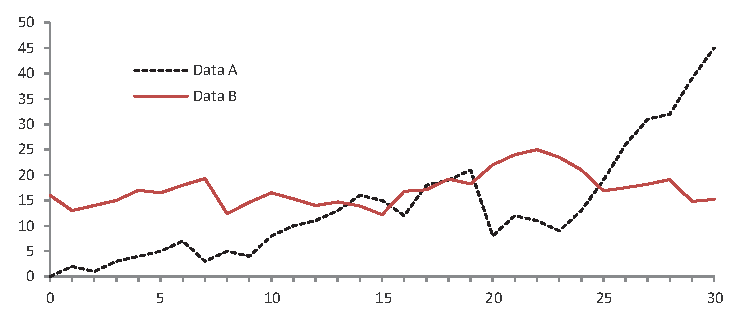
\includegraphics[width=\textwidth]{fig1.eps}
\caption{A figure caption is always placed below the illustration.
Please note that short captions are centered, while long ones are
justified by the macro package automatically.} \label{fig1}
\end{figure}
